% =========================================================================== %
% The Scout Client
% =========================================================================== %

\ifx\wholebook\relax\else
  \documentclass[a4paper,10pt,twoside]{book}
  %=============================================================================%
% Common things, settings, packages to include
%=============================================================================%

\usepackage{graphicx}
\usepackage{color}
\usepackage{makeidx}
\usepackage{ifpdf}
\usepackage{verbatim}

% --------------------------------------------------------------------------- %
% Setting up stuff depeding on output format
% --------------------------------------------------------------------------- %

\ifpdf
  % special settings for pdf mode
  \usepackage[colorlinks]{hyperref}
  \usepackage{courier}
  
  \hypersetup{
    colorlinks,
    linkcolor=darkblue,
    citecolor=darkblue,
    pdftitle={The Eclipse Scout Book},
    pdfauthor={The Scout Community},
    pdfkeywords={Enterprise Framework, Eclipse, Java, Client-Side, Rich Client, Web Client, Mobile},
    pdfsubject={Computer Science}
  }
  
  \usepackage{caption}
  \captionsetup{margin=10pt,font=small,labelfont=bf}
\else
  % special stuff for html mode
  \usepackage[tex4ht]{hyperref}
\fi

% --------------------------------------------------------------------------- %
% Setting up printing range
% --------------------------------------------------------------------------- %

\parindent 1cm
\parskip 0.2cm
\topmargin 0.2cm
\oddsidemargin 1cm
\evensidemargin 0.5cm
\textwidth 15cm
\textheight 21cm

% --------------------------------------------------------------------------- %
% Setting up listings
% --------------------------------------------------------------------------- %

\usepackage{listings}
 
\definecolor{darkviolet}{rgb}{0.5,0,0.4}
\definecolor{darkgreen}{rgb}{0,0.4,0.2} 
\definecolor{darkblue}{rgb}{0.1,0.1,0.9}
\definecolor{darkgrey}{rgb}{0.5,0.5,0.5}
\definecolor{lightblue}{rgb}{0.4,0.4,1}
\definecolor{lightgray}{rgb}{0.97,0.97,0.97}

\renewcommand{\lstlistlistingname}{List of Listings}

% general settings
\lstset{
  basicstyle=\small\ttfamily,
  columns=fullflexible,
  breaklines=true,
  breakindent=10pt,
  prebreak=\mbox{{\color{blue}\tiny$\searrow$}},
  postbreak=\mbox{{\color{blue}\tiny$\rightarrow$}},
  showstringspaces=false,
  backgroundcolor=\color{lightgray}
}

% settings for xml files
\lstdefinelanguage{xml}
{
  commentstyle=\color{darkgrey}\upshape,
  morestring=[b]",
  morestring=[s]{>}{<},
  morecomment=[s]{<?}{?>},
  stringstyle=\color{black},
  identifierstyle=\color{darkblue},
  keywordstyle=\color{cyan},
  morekeywords={xmlns,name,point,factory,class}% list your attributes here
}

% settings for ini files
\lstdefinelanguage{ini}
{
  morecomment=[f][\color{darkgrey}\upshape][0]\#, % # is comment iff it's the first char on the line
  stringstyle=\color{black}
}

% default settings (for java files)
\lstset{
  language=Java,
  emphstyle=\color{red}\bfseries,
  keywordstyle=\color{darkviolet}\bfseries,
  commentstyle=\color{darkgreen},
  morecomment=[s][\color{lightblue}]{/**}{*/},
  stringstyle=\color{darkblue},
}

% --------------------------------------------------------------------------- %
% cross reference macros
% --------------------------------------------------------------------------- %
\newcommand{\applabel}[1]{\label{apx:#1}}
\newcommand{\chalabel}[1]{\label{cha:#1}}
\newcommand{\seclabel}[1]{\label{sec:#1}}
\newcommand{\lstlabel}[1]{\label{lst:#1}}
\newcommand{\figlabel}[1]{\label{fig:#1}}
\newcommand{\tablabel}[1]{\label{tab:#1}}

\newcommand{\appref}[1]{Appendix~\ref{apx:#1}}
\newcommand{\charef}[1]{Chapter~\ref{cha:#1}\xspace}
\newcommand{\secref}[1]{Section~\ref{sec:#1}}
\newcommand{\lstref}[1]{Listing~\ref{lst:#1}\xspace}
\newcommand{\figref}[1]{Figure~\ref{fig:#1}\xspace}
\newcommand{\tabref}[1]{Table~\ref{tab:#1}\xspace}

% --------------------------------------------------------------------------- %
% graphics paths
% --------------------------------------------------------------------------- %
\graphicspath{
  {figures/}
  {Introduction/figures/}
}

%=============================================================================%

  \pagestyle{headings}
  \graphicspath{{figures/} {../figures/}}
  \begin{document}
  \sloppy
\fi


% =========================================================================== %
\chapter{Overview}
\chalabel{client_overview}

needs text
  
\noindent Existing Documentation
\begin{itemize}
  \item concept wiki \url{http://wiki.eclipse.org/Scout/Concepts/Client_Plug-In}
\end{itemize}

% --------------------------------------------------------------------------- %
\section{Client Model}
needs text

\noindent Existing Documentation
\begin{itemize}
  \item wiki concept \url{http://wiki.eclipse.org/Scout/Concepts/Client_Plug-In#Component_Model}
  \item concept wiki \url{http://wiki.eclipse.org/Scout/Concepts/ClientSession}
\end{itemize}

  * client session
  * ui
  * other
  
% --------------------------------------------------------------------------- %
\section{Client Server Communication}
needs text

% --------------------------------------------------------------------------- %
\section{UI Technologies}
needs text

\noindent Existing Documentation
\begin{itemize}
  \item wiki concept \url{http://wiki.eclipse.org/Scout/Concepts/Client_Plug-In#Separation_of_UI_and_GUI}
\end{itemize}
  
  * swing
  * swt
  * rap

% =========================================================================== %
\chapter{Shared Components}
needs text
  
% --------------------------------------------------------------------------- %
\section{Texts / i18n / NLS Support}
needs text

\noindent Existing Documentation
\begin{itemize}
  \item concept wiki: \url{http://wiki.eclipse.org/Scout/Concepts/Texts}
  \item forum: \url{http://www.eclipse.org/forums/index.php/t/319136/}
  \item forum: \url{http://www.eclipse.org/forums/index.php/t/326343/}
  \item forum: overwriting texts provided by scout \url{http://www.eclipse.org/forums/index.php/t/308273/}
  \item forum: additional text provider service \url{http://www.eclipse.org/forums/index.php/t/317565/}
  \item forum: changing default language for scout apps \url{http://www.eclipse.org/forums/index.php/t/367177/}
  \item forum: export/import not possible: \url{http://www.eclipse.org/forums/index.php/t/326320/}
  \item forum: usage counts for text entries: \url{http://www.eclipse.org/forums/index.php/t/261235/}
\end{itemize}

% --------------------------------------------------------------------------- %
\section{Icons}
needs text

\noindent Existing Documentation
\begin{itemize}
  \item how-to wiki \url{http://wiki.eclipse.org/Scout/HowTo/3.8/Add_an_icon}
  \item how-to wiki \url{http://wiki.eclipse.org/Scout/HowTo/3.8/Exchange_Default_Images}
\end{itemize}

% --------------------------------------------------------------------------- %
\section{Codes and Code Types}
needs text

\noindent Existing Documentation
\begin{itemize}
  \item how-to wiki: \url{http://wiki.eclipse.org/Scout/Tutorial/3.8/Minicrm/Code_Types}
  \item concept wiki \url{http://wiki.eclipse.org/Scout/Concepts/CodeType}
  \item forum: codes from database \url{http://www.eclipse.org/forums/index.php/t/282531/}
\end{itemize}

  * codes and codetypes
  * static code types
  * dynamic code types
  * hierarchical code types

% --------------------------------------------------------------------------- %
\section{Lookup Calls and Services}
needs text
 
\noindent Existing Documentation
\begin{itemize}
  \item presentation: \url{http://wiki.eclipse.org/images/c/c9/20111102_EclipseConEurope2011-EclipseScout-DiscoverThePotential.pdf}
  \item concept wiki: \url{http://wiki.eclipse.org/Scout/Concepts/LookupCall}
  \item forum: \url{http://www.eclipse.org/forums/index.php/t/279108/}
\end{itemize}

  * lookup call
  * lookup service
  * sqllookup service

% --------------------------------------------------------------------------- %
\section{Permissions}

needs text, topic is relevant for client, server, and security. what to present where to be decided

\noindent Existing Documentation
\begin{itemize}
  \item how-to wiki: \url{http://wiki.eclipse.org/Scout/HowTo/3.8/Create_Permissions}
  \item concept wiki: \url{http://wiki.eclipse.org/Scout/Concepts/Permission}
  \item forum: \url{http://www.eclipse.org/forums/index.php/t/243966/}
\end{itemize}

% --------------------------------------------------------------------------- %
\section{Form Data Objects}
needs text, explain that form data objects are data transfer objects

\noindent Existing Documentation
\begin{itemize}
  \item form data/dto \url{http://www.eclipse.org/forums/index.php/t/169334/}
\end{itemize}

\subsection{Data Binding}
needs text, this is about Form Data Export and Import

\subsection{Automatic Updates by the Scout SDK}
needs text

\subsection{Manual Form Data Updates}
needs text

% =========================================================================== %
\chapter{Client components}
needs text

% --------------------------------------------------------------------------- %
\section{Overview}

needs text
\begin{figure}[!htb]
\centering
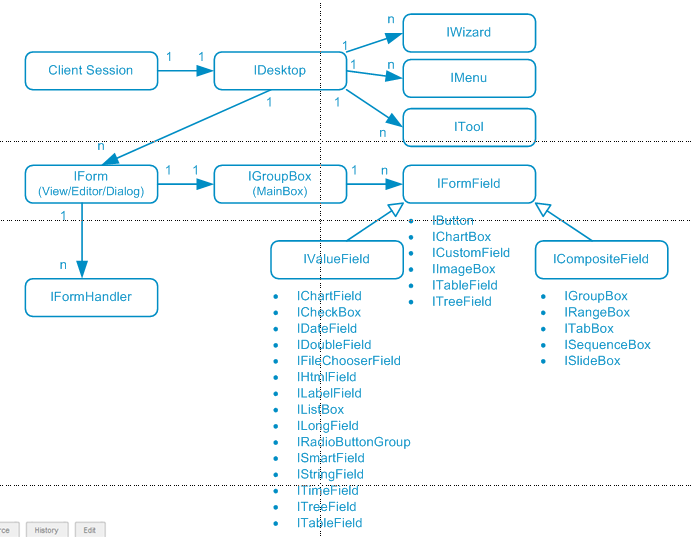
\includegraphics[width=0.8\textwidth]{scoutclientmodel.png}
\caption{A class diagram for the Scout's client model.}
\label{fig:scoutclientmodel}
\end{figure}

% --------------------------------------------------------------------------- %
\section{Splash Screen}
needs text

% --------------------------------------------------------------------------- %
\section{Login Box}
needs text

% --------------------------------------------------------------------------- %
\section{Client Session}
needs text

% --------------------------------------------------------------------------- %
\section{Desktop}
needs text

\noindent Existing Documentation
\begin{itemize}
  \item concept wiki \url{http://wiki.eclipse.org/Scout/Concepts/Desktop}
\end{itemize}

\subsection{Info Dialog}
needs text

\subsection{Toolbar}
needs text

\noindent Existing Documentation
\begin{itemize}
  \item forum: feature request \url{http://www.eclipse.org/forums/index.php/t/366440/}
  \item concept wiki \url{http://wiki.eclipse.org/Scout/Concepts/Tool}
\end{itemize}

\subsection{Status Line}
needs text

% --------------------------------------------------------------------------- %
\section{Menus}
needs text

\noindent Existing Documentation
\begin{itemize}
  \item concept wiki \url{http://wiki.eclipse.org/Scout/Concepts/Menu}
  \item forum: hard coded swt menues \url{http://www.eclipse.org/forums/index.php/t/236071/}. is this still an issue with scout kepler?
\end{itemize}

% --------------------------------------------------------------------------- %
\section{Outlines}
needs text

\noindent Existing Documentation
\begin{itemize}
  \item concept wiki \url{http://wiki.eclipse.org/Scout/Concepts/Outline}
\end{itemize}

% --------------------------------------------------------------------------- %
\section{Tools}
needs text

	
% --------------------------------------------------------------------------- %
\section{Forms}
needs text

\noindent Existing Documentation
\begin{itemize}
  \item concept wiki \url{http://wiki.eclipse.org/Scout/Concepts/Form}
  \item concept wiki form handler\url{http://wiki.eclipse.org/Scout/Concepts/Form_Handler}
  \item how-to wiki \url{http://wiki.eclipse.org/Scout/HowTo/3.8/Open_a_Form_in_a_View}
  \item forum: layout manager \url{http://www.eclipse.org/forums/index.php/t/404048/}
  \item forum: life cycle \url{http://www.eclipse.org/forums/index.php/t/369890/}
\end{itemize}

	* form validation

% --------------------------------------------------------------------------- %
\section{Form Fields}
needs text

Every Scout form contains one or several form fields.
Form fields therefor represent the basic building blocks of a forms content. 
Depending on their nature, form fields can display information, accept user input or act as container holding inner form fields.
As such container fields can hold inner container fields it is possible to create forms that meet compolex requirements.

\noindent Existing Documentation
\begin{itemize}
  \item concept wiki (links) \url{http://wiki.eclipse.org/Scout/Concepts/Client_Plug-In#Form_fields}
  \item concept wiki screenshots \url{http://wiki.eclipse.org/Scout/Concepts/Field}
\end{itemize}

% --------------------------------------------------------------------------- %
\section{Trees}
needs text

    * tree nodes
	* tree form
	* tree field

	
% --------------------------------------------------------------------------- %
\section{Pages}
needs text

\noindent Existing Documentation
\begin{itemize}
  \item how-to wiki: \url{http://wiki.eclipse.org/Scout/HowTo/3.8/Display_images_in_a_table_page}	
  \item concept wiki: \url{http://wiki.eclipse.org/Scout/Concepts/Page}
  \item forum: pages linking to forms \url{http://www.eclipse.org/forums/index.php/t/367595/}
  \item forum: changing page icons \url{http://www.eclipse.org/forums/index.php/t/262151/}
\end{itemize}

    * page with table
	* page with nodes

	
% --------------------------------------------------------------------------- %
\section{Search Forms}
needs text

\noindent Existing Documentation
\begin{itemize}
  \item forum: position of search form \url{http://www.eclipse.org/forums/index.php/t/353895/}
  \item forum: statement builder stuff \url{http://www.eclipse.org/forums/index.php/t/165805/}
\end{itemize}

% --------------------------------------------------------------------------- %
\section{Tables}
needs text

\noindent Existing Documentation
\begin{itemize}
  \item forum: editable column \url{http://www.eclipse.org/forums/index.php/t/220019/}
  \item forum: default visibility of columns \url{http://www.eclipse.org/forums/index.php/t/166052/}
  \item forum: row deletion \url{http://www.eclipse.org/forums/index.php/t/210744/}
\end{itemize}

	* context menues
	* editable tables
    * column types

\subsection{Image Columns}
needs text

\noindent Existing Documentation
\begin{itemize}
  \item forum: \url{http://www.eclipse.org/forums/index.php/t/369626/}
\end{itemize}

\subsection{HTML inside Table Cells}
needs text

\noindent Existing Documentation
\begin{itemize}
  \item forum: \url{http://www.eclipse.org/forums/index.php/t/370714/}
  \item forum: summary row \url{http://www.eclipse.org/forums/index.php/t/235749/}
\end{itemize}

\subsection{Table Status Bar}
nees text

\noindent Existing Documentation
\begin{itemize}
  \item forum: \url{http://www.eclipse.org/forums/index.php/t/367326/}
\end{itemize}

\subsection{Injecting Columns at Runtime}
needs text

\noindent Existing Documentation
\begin{itemize}
  \item forum: \url{http://www.eclipse.org/forums/index.php/t/364715/}
  \item forum : dynamic columns \url{http://www.eclipse.org/forums/index.php/t/216731/}
\end{itemize}

% --------------------------------------------------------------------------- %
\section{Workflows and Wizards}
Needs text

\noindent Existing Documentation
\begin{itemize}
  \item concept wiki \url{http://wiki.eclipse.org/Scout/Concepts/Wizard}
  \item forum: \url{http://www.eclipse.org/forums/index.php/t/391607/}
  \item forum: \url{http://www.eclipse.org/forums/index.php/t/382579/}
  \item forum: \url{http://www.eclipse.org/forums/index.php/t/366971/}
\end{itemize}


% =========================================================================== %
\chapter{Form Fields}
\chalabel{fields}

Every Scout form contains one or several form fields.
Form fields therefor represent the basic building blocks of a forms content. 
Depending on their nature, form fields can display information, accept user input or act as container holding inner form fields.
As such container fields can hold inner container fields it is possible to create forms that meet compolex requirements.

\noindent Existing Documentation
\begin{itemize}
  \item concept wiki (links) \url{http://wiki.eclipse.org/Scout/Concepts/Client_Plug-In#Form_fields}
  \item concept wiki screenshots \url{http://wiki.eclipse.org/Scout/Concepts/Field}
\end{itemize}

% --------------------------------------------------------------------------- %
\section{Common Aspects}
needs text

\noindent Existing Documentation
\begin{itemize}
  \item forum: label position \url{http://www.eclipse.org/forums/index.php/t/369109/}
\end{itemize}

* model component
* ui component
* extension point registration

* model
* label
* value
* exec methods
* field validation


% =========================================================================== %
\chapter{Simple Widgets}
\chalabel{simplewidgets}

This chapter presents the most commonly used Scout widgets.
Based on the Scout widget demo application provided with this book.
 
Except for the Message box at the end of this chapter the widgets discussed are all Scout form fields. 
For each field, example use cases are described. 
In addition, a screenshot of the corresponding form in the widget application illustrates these use cases.
Finally, exemplary code snippets taken from the widget application close the loop to the actual implementation of these widgets in the applications source code.


\begin{figure}
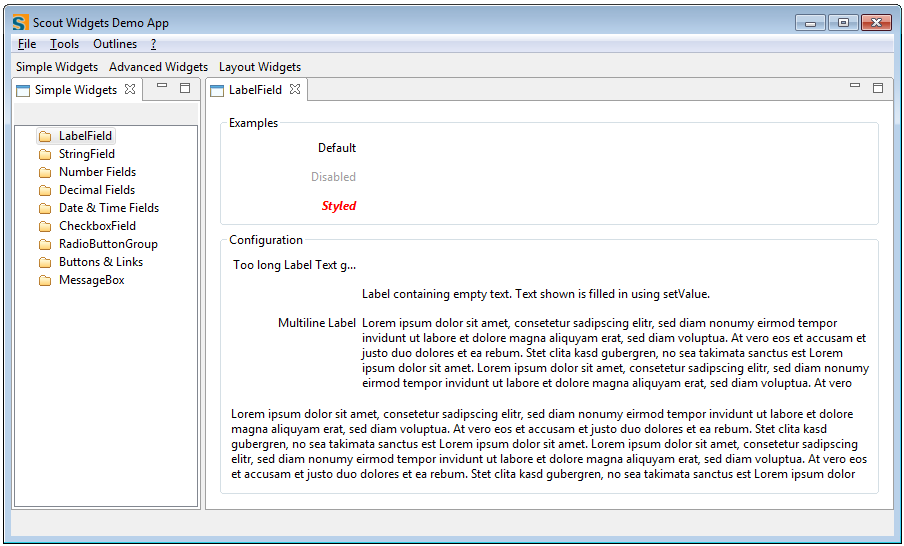
\includegraphics[width=15cm]{widgetapp_swt.png}
\caption{Scout fields and example use cases. 
In the examples section of the form the standard usage of label fields is shown.
To display text over the whole width of a column or in the area right to the label use method \java{setValue} as shown in the configuration section of the form.}
\figlabel{widgetapp_swt}
\end{figure}

\begin{figure}
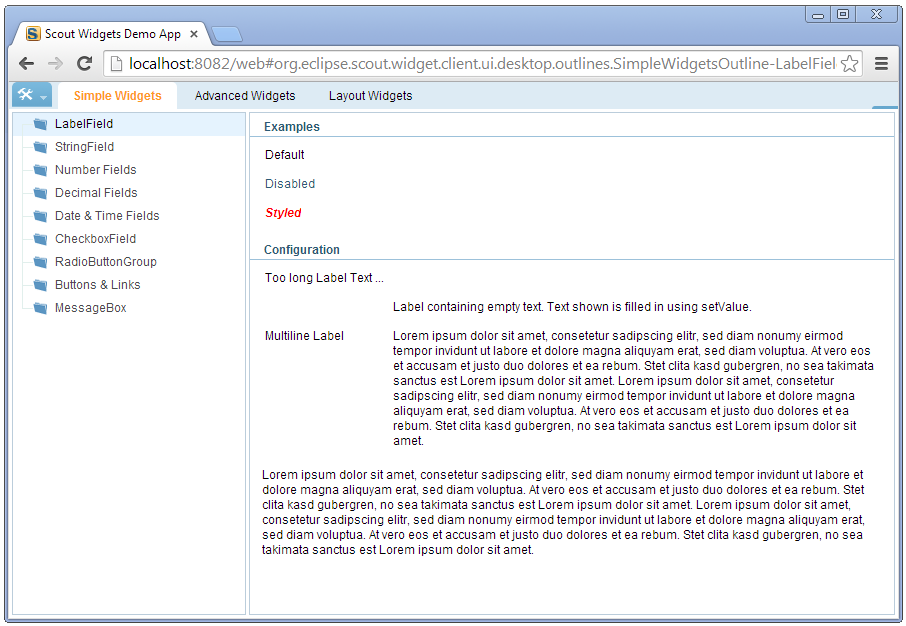
\includegraphics[width=15cm]{widgetapp_web.png}
\caption{Scout fields and example use cases. 
In the examples section of the form the standard usage of label fields is shown.
To display text over the whole width of a column or in the area right to the label use method \java{setValue} as shown in the configuration section of the form.}
\figlabel{widgetapp_web}
\end{figure}

\begin{figure}
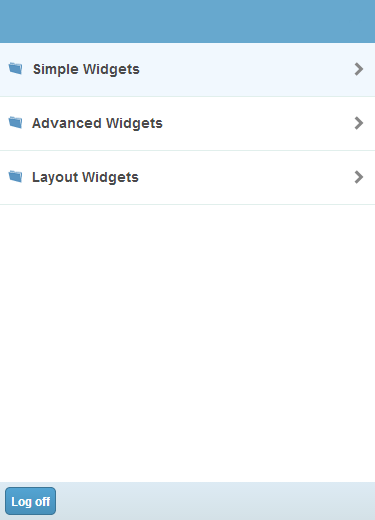
\includegraphics[width=5cm]{widgetapp_mobile1.png}
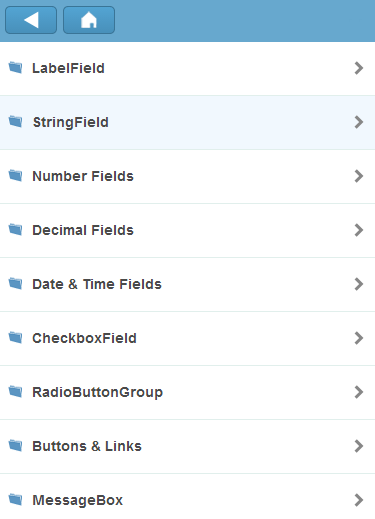
\includegraphics[width=5cm]{widgetapp_mobile2.png}
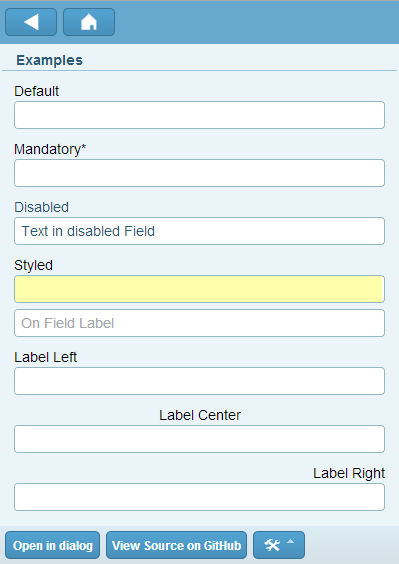
\includegraphics[width=5cm]{widgetapp_mobile3.png}
\caption{Scout fields and example use cases. 
In the examples section of the form the standard usage of label fields is shown.
To display text over the whole width of a column or in the area right to the label use method \java{setValue} as shown in the configuration section of the form.}
\figlabel{widgetapp_web}
\end{figure}

% --------------------------------------------------------------------------- %
\section{Label Fields}

Label fields are used to place a read only text anywhere in a Scout form. 
As shown in the configuration section of \figref{labelfield} such texts can occupy the typical area assigned to a label field on the left, the area typically assigned to data entry on the right or on both sides.
The form shown in \figref{labelfield} is implemented in class \java{LabelFieldForm} of the Scout widget application.

\begin{figure}
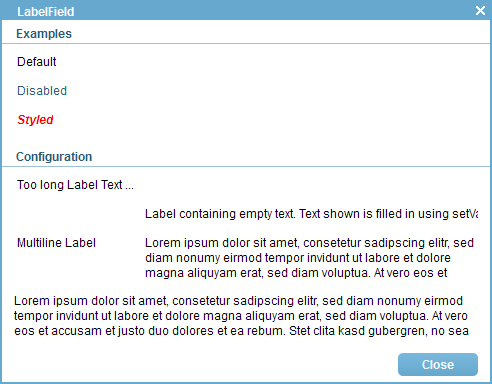
\includegraphics[width=10cm]{labelfield.png}
\caption{Scout fields and example use cases. 
In the examples section of the form the standard usage of label fields is shown.
To display text over the whole width of a column or in the area right to the label use method \java{setValue} as shown in the configuration section of the form.}
\figlabel{labelfield}
\end{figure}

To set the label text in the default area method \java{getConfiguredLabel} is used. 
If the label text is too long for the reserved area the label gets truncated with trailing \dots.
The complete label text is then shown in a tooltip.

Also, a number of \java{getConfiguredLabel*} styling properties exist for labels.
This is not only true for the label field itself but for any form field derived from \java{AbstractFormField}.
Most of these styling properties can directly be set in the Scout Object Properties view.
A subset of these properties are shown in the list below.

\begin{itemize}
  \item Label Position
  \item Label Horizontal Alignment
  \item Label Foreground Color
  \item Label Background Color
  \item Label Font
\end{itemize}

\lstinputlisting[
  label=\lstlabel{field.label.value},
  caption=A simple LabelField.,
  index={AbstractLabelField,Label Field},
  linerange={181-194},
  float
]
{../code/widgets/org.eclipse.scout.widget.client/src/org/eclipse/scout/widget/client/ui/forms/LabelFieldForm.java}

To display text in the right hand area an empty string can be used as label text and the text for the value area of the label field can be set with method \java{setValue} in method \java{execInitField} according to \lstref{field.label.value}.

\lstinputlisting[
  label=\lstlabel{field.label.multiline},
  caption=A label field displaying multi-line text that covers the whole width of a column.,
  index={AbstractLabelField,Label Field},
  linerange={223-251},
  float
]
{../code/widgets/org.eclipse.scout.widget.client/src/org/eclipse/scout/widget/client/ui/forms/LabelFieldForm.java}

To display multiline text across both the label and the value area a combination of label field properties has to be used.
See \lstref{field.label.multiline} for the configuration used in the last label field shown in \figref{labelfield}.

% --------------------------------------------------------------------------- %
\section{String Fields}

String fields are used to enter simple text strings. 
In addition, string fields are also useful to enter multiline text or capture masked input.
The form shown in \figref{stringfield} is implemented in class \java{StringFieldForm} of the Scout widget application.

\begin{figure}
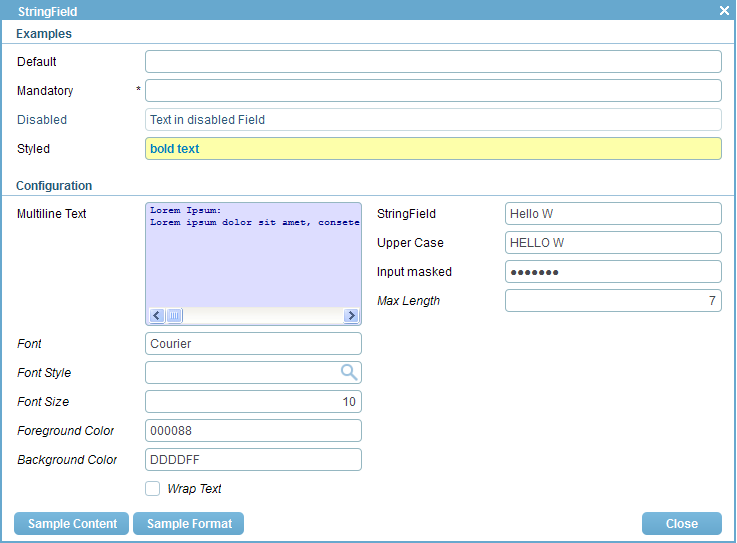
\includegraphics[width=15cm]{stringfield.png}
\caption{String fields and example use cases.
Text content shown in disabled fields can be read and copied to the clipboard, but not edited.
In multi line string fields the text can be displayed as entered or the text may be wrapped to fit into the available column with.}
\figlabel{stringfield}
\end{figure}

Some of the most typical use cases for string fields are represented in the examples section of \figref{stringfield}.
In the configuration section of the form a multiline text field is shown.
As in the case of the label text, font and color styling possibilities are available for the text shown in a string field. 
Clicking on the \button{Sample Format} and on the \button{Sample Content} prefills some of the fields to create the effect shown in \figref{stringfield}.

In the case of multi line string fields, the field can be configured to either display text lines as they have been entered or wrapped to fit into the available width of the field. 
This property can be set with the string field's method \java{getConfiguredWrapText} or dynamically with method \java{setWrapText}. 
Please note that changing this property dynamically at runtime currently only works with the SWT and the Swing rendering components.

\lstinputlisting[
  label=\lstlabel{field.string.masked},
  caption=A masked string field.,
  index={AbstractStringField,String Field},
  linerange={522-535},
  float
]
{../code/widgets/org.eclipse.scout.widget.client/src/org/eclipse/scout/widget/client/ui/forms/StringFieldForm.java}

Additional use cases for the string field are shown in the right column of the configuration section of the string field demo form. 
Specific string fields are located for the default case, a string field only accepting upper case letters, and a masked field. 
To code to represent the masked string field is provided in \lstref{field.string.masked}.
Independent of what the user is typing the masked field keeps the entered content visually hidden. 
In contrast to all other forms of string fields, the content cannot be copied to the system clipboard.
It can only be accessed programmatically with the \java{getValue} method of the string field.

String fields also allow for the configuration of the maximum length of the text that can be entered into the field. 
In its default configuration, a maximum number of 4'000 characters can be entered into a string field. 
Using method \java{setMaxLength} this limit can be updated dynamically at runtime. 
Alternatively, this limit can also be set in method \java{getConfiguredMaxLength}. 

% --------------------------------------------------------------------------- %
\section{Number Fields}

For entering numbers, Scout provides three different fields.
Depending on the valid range of numbers that may be entered, an integer field, a long field or a big integer field best matches the given use case.
These fields are represented by the classes \java{AbstractIntegerField}, \java{AbstractLongField} and \java{AbstractBigIntegerField}, each one of them extinding class \java{AbstractNumberField}.

\begin{figure}
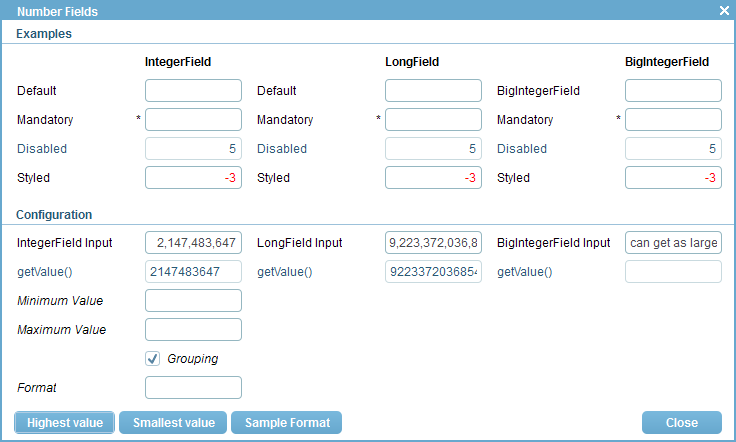
\includegraphics[width=15cm]{numberfield.png}
\caption{Number fields and example use cases.
Distinct number fields are available for \java{Integer}, a \java{Long} or a \java{BigInteger} value classes.
}
\figlabel{numberfield}
\end{figure}

The form \java{NumberFieldsForm} of the Scout widget application shown in \figref{numberfield} contains examples for all three number field types.
Separate buttons are available to demonstrate the use of the minimum and the maximum value a number field can hold.
In the case of the \field{BigInteger}, arbitrarily large or small values may be entered. 
See \lstref{field.integer.input} for the code corresponding to the input integer field in the configuration section of the example form.

\lstinputlisting[
  label=\lstlabel{field.integer.input},
  caption=A simple Integer field.,
  index={AbstractIntegerField,Integer Field},
  linerange={511-519},
  float
]
{../code/widgets/org.eclipse.scout.widget.client/src/org/eclipse/scout/widget/client/ui/forms/NumberFieldsForm.java}

As already indicated by the class names of the three number fields, the fields serve to enter values that fit into the ranges defined by the Java classes \java{Integer}, \java{Long} and \java{BigInteger}.
To further restrict the bounds of valid numbers you may use the methods \java{getConfiguredMinValue} and \java{getConfiguredMaxValue}.
The effect of setting such bounds can be tested by entering values into the \field{Minimum Value} and the \field{Maximum Value} of the example form.
If, for example, a minimum value of 0 is entered in the \field{Minimum Value} and the user tries to enter the value -1 into one of the input fields, an error marker becomes visible on the input field. 
A tooltip with the text ''The value is too small; must be between 0 \dots'' further explains the issue to the user.
In such a case the value entered into the user interface is not propagated to the number field's value.
This is why the read only \field{getValue()} is not updated in such a case.

To textually format the entered numbers the grouping number field property can be used. 
In the example form the \checkbox{Grouping} can be used to control this property.
Ticking/unticking this checkbox will affect the three number input fields in the configuration section of the example form.

More extensive options to specify the formatting of the numbers is provided by the method \java{setFormat} of class \java{AbstractNumberField}. 
Method \java{setFormat} is accepting an argument of the Java class \java{DecimalFormat}. 
To demonstrate an example for such a format click on \button{Sample Format} in the example form. 
For more information please consult the Javadoc for class \java{DecimalFormat}.

% --------------------------------------------------------------------------- %
\section{Decimal Fields}

Scout provides two different form fields for entering decimal values. 
Depending on the required precision and range of values to be entered a double field or a big decimal field can be used. 
The two field types are represented by Scout's classes \java{AbstractDoubleField} and \java{AbstractBigDecimalField} and can hold values of the Java types \java{Double} and \java{BigDecimal} respectively. 
Both the double and the big decimal field extend class \java{AbstractDecimalField} which in turn extends class \java{AbstractNumberField}.

\begin{figure}
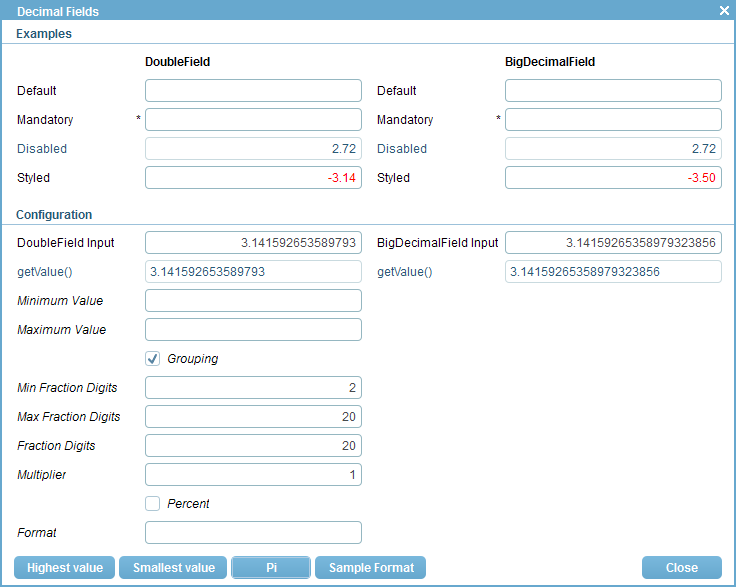
\includegraphics[width=15cm]{decimalfield.png}
\caption{Decimal fields and example use cases.
Distinct number fields are available for the \java{Double} and \java{BigDecimal} value classes.
}
\figlabel{decimalfield}
\end{figure}

The example form shown in \figref{decimalfield} demonstrates the usage and some of the available options to configure Scout's decimal fields.
This example form is defined in class \java{DecimalFieldsForm} of the Scout widget application. 

\lstinputlisting[
  label=\lstlabel{field.double.styled},
  caption=A styled decimal field holding Java \java{Double} values. Negative values are shown in red,
  index={AbstractDoubleField,Double Field},
  linerange={313-337},
  float
]
{../code/widgets/org.eclipse.scout.widget.client/src/org/eclipse/scout/widget/client/ui/forms/DecimalFieldsForm.java}

The styled double field in the example section of the form displays negative values in red and postive values in the default black color. 
This behaviour is implemented in method \java{execChangedValue} according to \lstref{field.double.styled}. 
The sample value shown initially is provided in the \java{execInitField} method. 
Setting the red foreground color explicitely is needed in method \java{execInitField} as the \java{execChangedValue} is only triggered after the initial form is displayed on the screen. 

For displaying and storing the fraction digits of decimal values three different properties exist. 
Two of them, the \java{getConfiguredMinFractionDigits} and the \java{getConfiguredMinFractionDigits} affect the optical representation of the decimal value. 
To configure the amount of fraction digits that is effectively represented the property \java{getConfiguredFractionDigits} is used. 
The need for three different properties might not be immediately clear. 
To illustrate the concept, let us look at an example use case where a decimal field always has to display exactely 3 fraction digits. 
Should the user provide more fraction digits we would like to capture this additional information up to 5 fraction digits. 

To configure this behaviour the following settings for this decimal field may be used.

\begin{itemize}
  \item \textit{Min Fraction Digits}: 3
  \item \textit{Max Fraction Digits}: 3
  \item \textit{Fraction Digits}: 5
\end{itemize}

If the user enters the text ''3.141592653589793'' into this field and tabs to the next field, the field will then display the text ''4.142'' but actually hold the value 3.14159. 
And if the user just enters a ''3'', the field will display ''3.000'' and hold the value 3.0.

Decimal fields can also be configured to enter percentages in a convenient way. 
For this use case the \property{Multiplier} can be set to 100 and the \property{Multiplier} to \java{true}. 
If the user now enters ''5'' into such a decimal field, it will show the text ''5\%'' and hold the value 0.05.

As in the case of number fields more extensive options to specify the formatting of the numbers is provided by \java{setFormat} method of the decimal field. 
Method \java{setFormat} is accepting an argument of the Java class \java{DecimalFormat}. 
To demonstrate an example for such a format click on \button{Sample Format} in the example form. 
For more information please consult the Javadoc for class \java{DecimalFormat}.

% --------------------------------------------------------------------------- %
\section{Date and Time Fields}

To work with date and time values Scout offers three dinstinct form fields. 
The \java{AbstractDateField} allows the user to enter a date and the \java{AbstractTimeField} is used to enter a time. 
The third field \java{AbstractDateTimeField} combines date and time entry into a single form field. 
Both classes \java{AbstractTimeField} and \java{AbstractDateTimeField} are extending the \java{AbstractDateField} field.

\begin{figure}
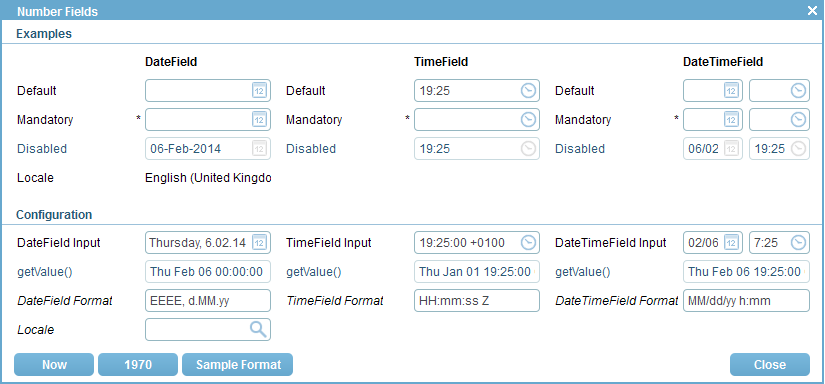
\includegraphics[width=15cm]{datetimefield.png}
\caption{Example use cases for a date, a time and a combined date/time field.
}
\figlabel{datetimefield}
\end{figure}

The form \java{DateTimeFieldsForm} of the Scout widget application shown in \figref{datetimefield} contains examples for the date and time fields of Scout.
Separate buttons are available to provide samle values and to demonstrate the formatting options for displaying date and time values.
Displaying dates and times is highly depending on the used locale.
That is why the currently used locale is shown in the example section of the form.

To enter date and time values the user can either click on the date and time icons/buttons provided by the fields or directly enter text into the fields. 
For entering dates the key arrows provide a number of shortcuts. 
Entering the currnt date can be done by pressing the \key{Up}. 
Once a day is entered in a date or a combined day time field, the \key{Up} and the \key{Down} can be used to step to the next/previous day. 
Simultaneously pressing the \key{Shift} or the \key{Ctrl} allows to step to the next/previous month or year.

\lstinputlisting[
  label=\lstlabel{field.datetime.disabled},
  caption=A disabled combined date time field initialized with the current time,
  index={AbstractDateTimeField,DateTime Field},
  linerange={427-446},
  float
]
{../code/widgets/org.eclipse.scout.widget.client/src/org/eclipse/scout/widget/client/ui/forms/DateTimeFieldsForm.java}

The code of the \java{DateTimeDisabledField} field shown in \lstref{field.datetime.disabled} represents the disabled combined date time in the example form. 
Before the form is opened Scout executes its \java{execInitField} method and sets the fields value to the current date and time. 

In the configuration section the local can be used at runtime to test the effect of the locale to displaying date and time fields. 
As changing the locale at runtime only works reliably in rich clients the field is only editable in the Swing or the SWT client. 
To specify the exact formatting of the displayed date and time values a specific format can be set in the \java{getConfiguredFormat} method of the date and time fields. 
Internally, Scout is using the provided string to create a Java \java{SimpleDateFormat} for formatting. 
Valid examples for the formatting are entered into the format fields of the example dialog by pressing the \button{Sample Formats}. 
The string ''EEEE'' shown in date field format field represents the day of the week as shown in configuration section of \figref{datetimefield}. 
As expected, the textual representation of the day of the week is depending on the used locale. 

% --------------------------------------------------------------------------- %
\section{Checkbox Fields}

Checkboxes can be used to enter/represent simple boolean values. 
In Scout, checkboxes are derived from class \java{AbstractCheckBox}. 

\begin{figure}
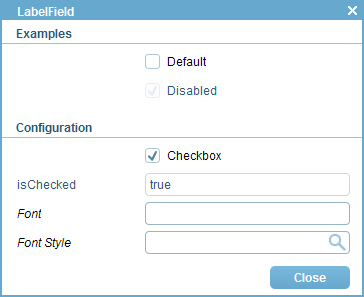
\includegraphics[width=7cm]{checkboxfield.png}
\caption{Check box field and example use cases.
}
\figlabel{checkboxfield}
\end{figure}

In the Scout widget application the use of checkboxes is demonstrated in the form \java{CheckboxFieldForm} that is shown in \figref{checkboxfield}.
Instead of the method \java{getValue} that is available on the other value fields, the method \java{isChecked} is provided.

\lstinputlisting[
  label=\lstlabel{field.checkbox.disabled},
  caption=A disabled check box field initialized with a checked state,
  index={AbstractCheckBox,Check Box},
  linerange={144-163},
  float
]
{../code/widgets/org.eclipse.scout.widget.client/src/org/eclipse/scout/widget/client/ui/forms/CheckboxFieldForm.java}

A coding example is provided in \lstref{field.checkbox.disabled} for the disabled check box. 
The initial value is set in method \java{execInitField} using the method \java{setChecked}.

% --------------------------------------------------------------------------- %
\section{Radio Button Fields}

With radio buttons the user can select a single element out of a number of distinct choices. 
For this, a number of radio buttons may be placed into a radio button group field where a radio button group extends class \java{AbstractRadioButtonGroup}.
The contained individual buttons are extending class \java{AbstractRadioButton}.

\begin{figure}
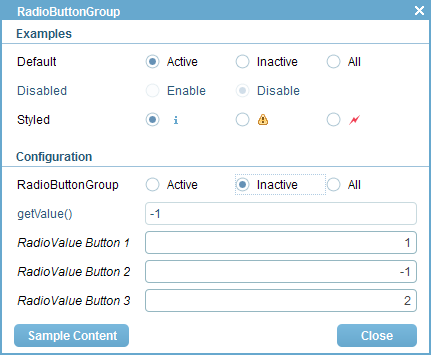
\includegraphics[width=9cm]{radiobuttonfield.png}
\caption{Radio buttons in a radio button group field and example use cases.
Assigning distinct values to the individual radio buttons allows to query the selected radio button.}
\figlabel{radiobuttonfield}
\end{figure}

\figref{radiobuttonfield} demonstrates the use of radio button groups in Scout. 
It is implemented in class \java{RadioButtonGroupFieldForm} of the Scout widget application. 
As shown in the example section of the form radio buttons may have labes and/or icons assigned. 
If the radio buttons have assigned individual values of the Java type \java{Long} the currently selected value may be obtained using the \java{getValue} method of the radio button group. 

\lstinputlisting[
  label=\lstlabel{field.radiobuttongroup.styled},
  caption=A complete radio button group with two radio buttons with individual radio values assigned,
  index={AbstractCheckBox,Check Box},
  linerange={289-329},
  float
]
{../code/widgets/org.eclipse.scout.widget.client/src/org/eclipse/scout/widget/client/ui/forms/RadioButtonGroupFieldForm.java}

The code representing the styled radio button group is provided in \lstref{field.radiobuttongroup.styled}. 
The type of the value that is returned by the \java{getValue} method is defined on the radio button group. 
In the provided listing, the \java{StyledGroupBox} is configured to return a value of the type \java{Long}. 
Consequently, the individual radio buttons are returning radio values of the type \java{Long} as well in the \java{getConfiguredRadioValue} methods.
The field \java{PlaceholderField} in the radio button group only serves layouting purposes. 
Without this placeholder field, the two radio buttons of the styled radio button group would be evenly distributed in the available space. 

% --------------------------------------------------------------------------- %
\section{Buttons and Links}

Buttons and links are used to trigger actions in Scout. 
Buttons come in two variations, normal push buttons and toggle buttons. 
While buttons have an associated label and/or icon, links can only have a label. 
Buttons extend class \java{AbstractButton} and links extend \java{AbstractLinkButton}. 

\begin{figure}
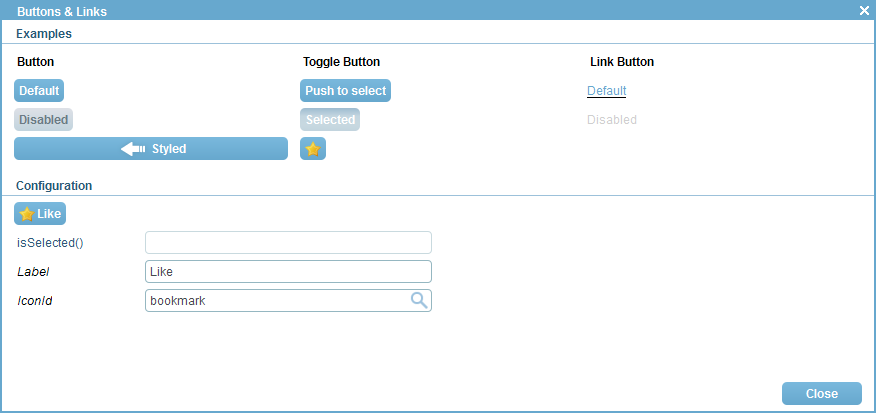
\includegraphics[width=15cm]{buttonlink.png}
\caption{Buttons and links may be placed on a Scout form to initiate actions.
Buttons may have an associated icon and/or a label.
Links only have a label.}
\figlabel{buttonlink}
\end{figure}

Example uses of buttons and links are shown in the form \java{ButtonLinkFieldsForm} of the Scout widget application shown in \figref{buttonlink}. 

\lstinputlisting[
  label=\lstlabel{field.button.styled},
  caption=A button with a label and an icon that horizontally streches over the whole column,
  index={AbstractButton,Button},
  linerange={208-231},
  float
]
{../code/widgets/org.eclipse.scout.widget.client/src/org/eclipse/scout/widget/client/ui/forms/ButtonLinkFieldsForm.java}

In it's simplest form a button just extends class \java{AbstractButton} and overrides \java{getConfiguredLabel} to set the label. 
The example in \lstref{field.button.styled} also has an icon assigned and stretches over the whole column width. 
In addition, the example button overrides method \java{getConfiguredProcessButton} to return \java{false}. 
This has the effect that buttons (and links) appear at the exact location where they are defined a field container. 
Otherwise, buttons (and links) are placed at the bottom of the container they are defined in. 

\lstinputlisting[
  label=\lstlabel{field.togglebutton},
  caption=A toggle button implementation that changes the label text depending on its toggled state,
  index={AbstractButton,Toggle Button},
  linerange={245-273},
  float
]
{../code/widgets/org.eclipse.scout.widget.client/src/org/eclipse/scout/widget/client/ui/forms/ButtonLinkFieldsForm.java}

The code of the default toggle button in the example form of the widget application is provided in \lstref{field.togglebutton}. 
To query the state of a toggle button method \java{isSelected} can be used. 

In the configuration section of the example form the use of mnemonics using the character \& is demonstrated. 
Please note, that this feature is not identically available across the different supported UI technologies. 
In the Swing UI shown in \figref{buttonlink} the label ''\&Toggle'' has the effect, that pressing the \altkey{T} key combination changes the toggle state of this button. 
In the case of the SWT UI the \key{alt} key is not necessary. 
Pressing the \key{T} changes the toggle state. 
In contrast to the Swing UI the letter 'T' is not underlined. 
To optically indicate shortcut letters in the SWT UI it is recommended to adapt the label from ''\&Toggle'' to ''[\&T]oggle''. 
The RAP UI does not currently support mnemonics on buttons. 

% --------------------------------------------------------------------------- %
\section{Message Boxes}

Message boxes are used to provide information to a user or ask the user simple yes/no questions. 
In Scout, class \java{MessageBox} provides a number of static convenience methods for this purpose. 
Additionally, message boxes are shown to the user in the case of a processing exception or a veto exception\footnote{
The processing exceptions type \java{ProcessingException} represents Scout's core exception class. 
The veto exception type \java{VetoException} is a direct subclass of the processing exception and is typically used in service calls for subjects with insuffiecient authorization. 
}. 

\begin{figure}
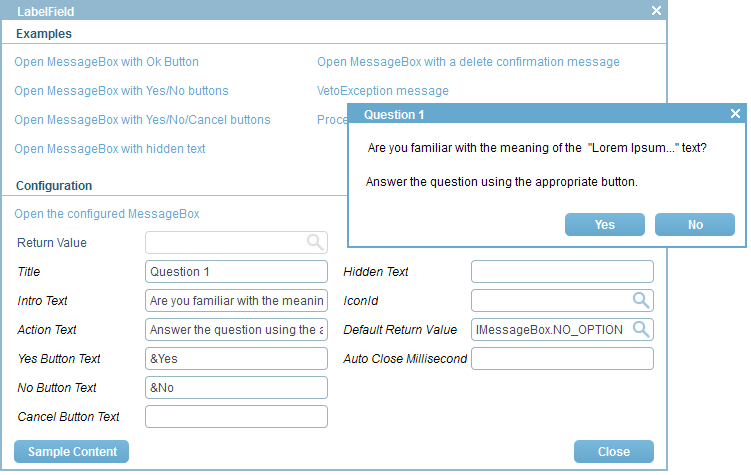
\includegraphics[width=14cm]{messagebox.png}
\caption{Message boxes are available for different use cases.
The message box shown in front is defined by the properties entered in the configuration section.}
\figlabel{messagebox}
\end{figure}

In the examples section of the \java{MessageBoxForm} form shown in \figref{messagebox} a number of links is provided. 
Clicking on any of these links opens a corresponding message box via the static convenience methods available with class \java{MessageBox}. 
For example, calling \java{MessageBox.showOkMessage(title, header, info)} opens a message box with a title, a header text and some additional information. 

\lstinputlisting[
  label=\lstlabel{field.openmessagebox},
  caption=Configuring and starting of a message box.,
  index={MessageBox,Configure a Message Box},
  linerange={434-453},
  float
]
{../code/widgets/org.eclipse.scout.widget.client/src/org/eclipse/scout/widget/client/ui/forms/MessageBoxForm.java}

In addition to the static convenience methods, message boxes can be configured to meet specific requirements by a number of parameters. 
These parameters are shown in \figref{messagebox} in the configuration section of the sample form \java{MessageBoxForm} of the Scout widget application.  
Clicking on the \button{Sample Content} will fill in example values for the message box parameters. 
The configured message box can them be started by clicking on the \link{Open the configured MessageBox}. 
This behaviour is implemented in the link's \java{execClickAction} method according to \lstref{field.openmessagebox}. 
The text below details the purpose of less evident message box properties.

Message box buttons only appear if an non-emtpy label text is assigned to the \property{Yes Button Text}, the \property{No Button Text} and \property{Cancel Button Text}. 
If the \property{hidden text} has a non-empty text assigned, an additional \button{Copy} will be added to the message box. 
An example use case is the case of elaborate error messages (or complete stack traces in cases where this does not negatively impact the application's security). 
Here the copy button allows to transport this text into the system clipboard. 
From the clipboard the user may decides to paste this text into an email to the companys help desk. 
The \property{default return value} specifies the return value of the message box if the box closes autmatically after the time provided in the \property{auto close millisecond} has passed. 
If the \property{auto close millisecond} is set to -1, the message box will not clause automatically. 

Once a message box is started with method \java{startMessageBox} the user interface is blocked until the user chooses any of the options or clicks the dialog away. 
The selected option is the provided by the method's return value. 
If the user closes the message box by hitting the \key{esc} or clicking on the icon to close a dialog, the start method of the message box will always return the value \java{CANCEL\_OPTION} of the \java{IMessageBox} interface.

% =========================================================================== %
\chapter{Advanced Widgets}
\chalabel{advancedwidgets}

% --------------------------------------------------------------------------- %
\section{List Box}
needs text

\begin{figure}
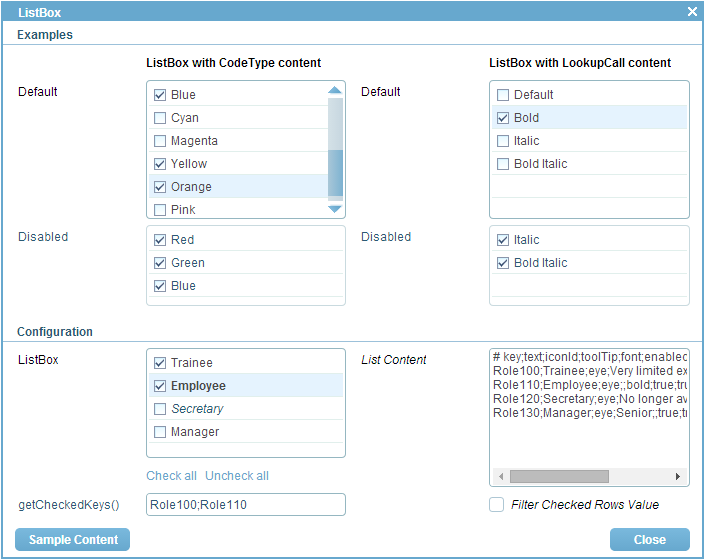
\includegraphics[width=14cm]{listbox.png}
\caption{List boxes and use cases.
More text.}
\figlabel{listbox}
\end{figure}

% --------------------------------------------------------------------------- %
\section{Tree Box}
needs text

\begin{figure}
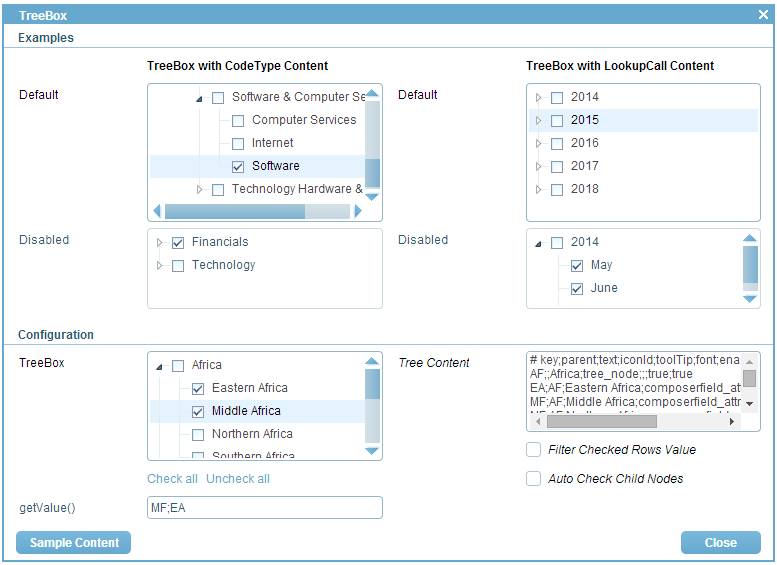
\includegraphics[width=14cm]{treebox.png}
\caption{Tree boxes and use cases.
More text.}
\figlabel{treebox}
\end{figure}

% --------------------------------------------------------------------------- %
\section{Smart Field}
needs text

\begin{figure}
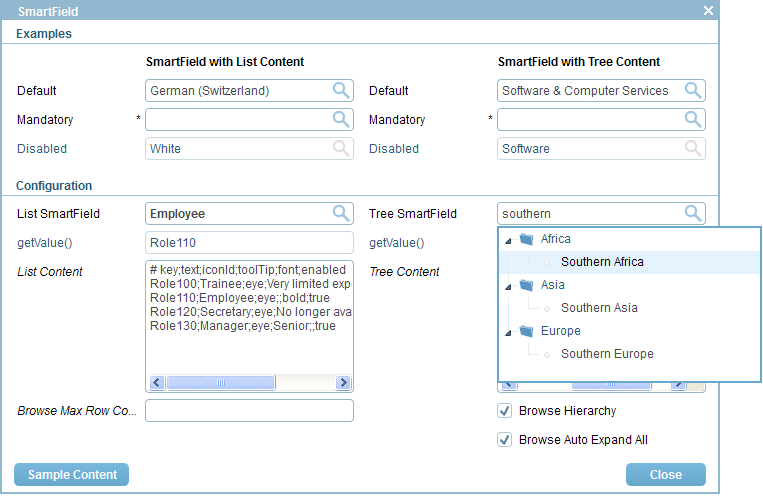
\includegraphics[width=14cm]{smartfield.png}
\caption{A smart field is a combo box on steroids.
Smart fields support ''search-as-you-type'' and are used to select a value out of a list or a tree.
The content values may come from a static set of values or can be dynamically provided at runtime.}
\figlabel{smartfield}
\end{figure}

\noindent Existing Documentation
\begin{itemize}
  \item presentation: \url{http://wiki.eclipse.org/images/c/c9/20111102_EclipseConEurope2011-EclipseScout-DiscoverThePotential.pdf}
  \item forum: \url{http://www.eclipse.org/forums/index.php/t/369542/}
\end{itemize}

\subsection{Menus}
Each smart field can have menus attached. The menus will be shown when the user clicks on the \emph{arrow} symbol next to the smart field. Figure \ref{fig:smartfield_menu} shows an example of a smart field along with a set of menus.
\begin{figure}[!htb]
\centering
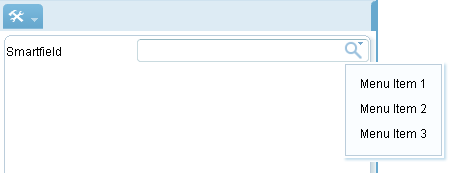
\includegraphics[width=0.8\textwidth]{smartfieldmenu.png}
\caption{Menus attached to a smart field.}
\label{fig:smartfield_menu}
\end{figure}

By default, the menus will only be shown if a value of the smart field has been selected. To show the menus even if the smart field is empty, one has to override the menu's \lstinline$getConfiguredEmptySpaceAction$ method:

\begin{lstlisting}[backgroundcolor=\color{white}]
@Override
protected boolean getConfiguredEmptySpaceAction() {
 return true;
}
\end{lstlisting}

% --------------------------------------------------------------------------- %
\section{Tree Field}
needs text

\begin{figure}
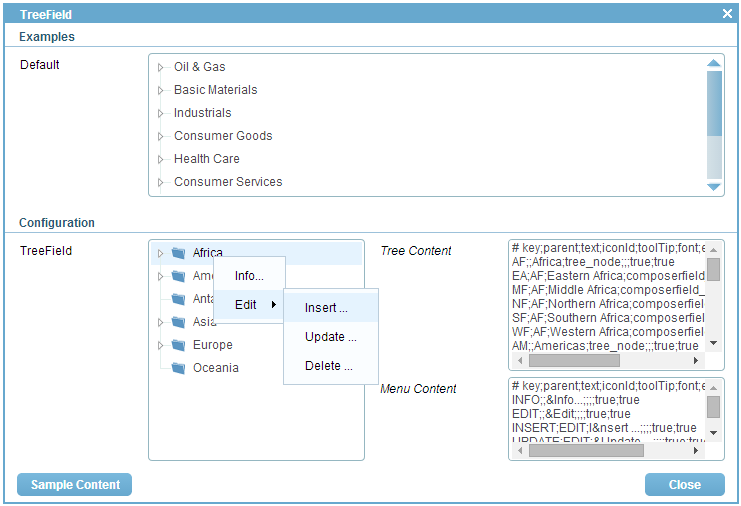
\includegraphics[width=15cm]{treefield.png}
\caption{Tree fields and example use cases.
More text.}
\figlabel{treefield}
\end{figure}

% --------------------------------------------------------------------------- %
\section{Table Field}
needs text

\begin{figure}
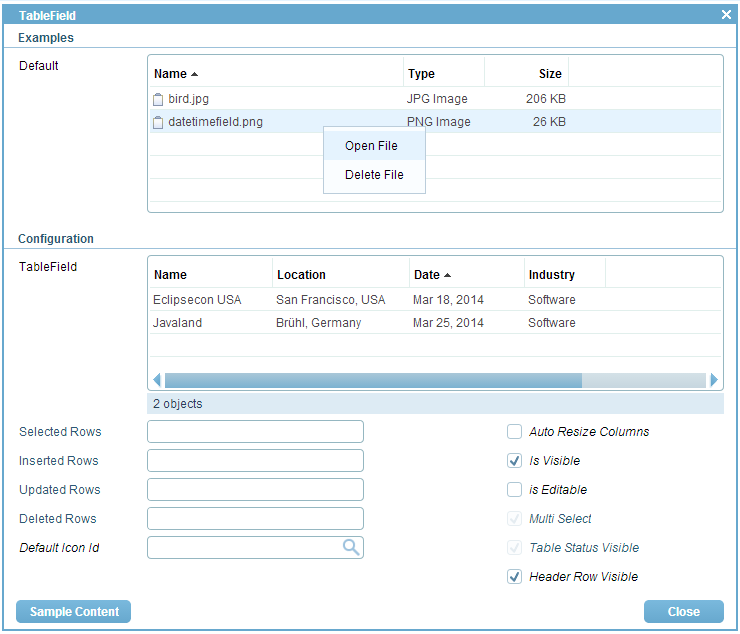
\includegraphics[width=15cm]{tablefield.png}
\caption{Table fields and example use cases.
More text.}
\figlabel{tablefield}
\end{figure}

\begin{figure}
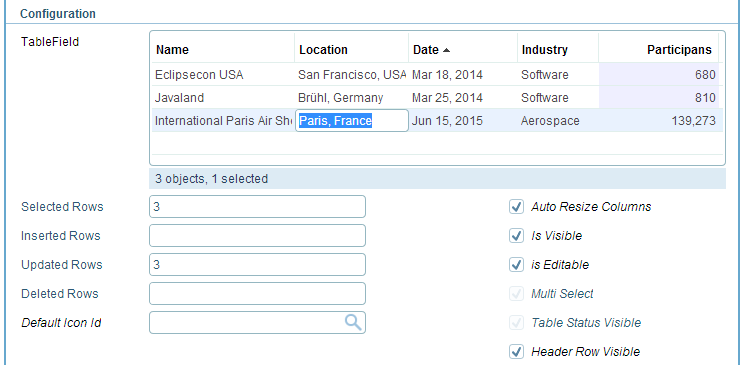
\includegraphics[width=15cm]{editabletablefield.png}
\caption{An editable table field.
More text.}
\figlabel{editabletablefield}
\end{figure}

\noindent Existing Documentation
\begin{itemize}
  \item wiki tutorial \url{http://wiki.eclipse.org/Scout/Tutorial/3.8/Minicrm/Table_Field}
  \item forum: \url{http://www.eclipse.org/forums/index.php/t/392053/}
  \item forum: load/save data \url{http://www.eclipse.org/forums/index.php/t/253311/}
\end{itemize}

% --------------------------------------------------------------------------- %
\section{Image Field}
needs text

\begin{figure}
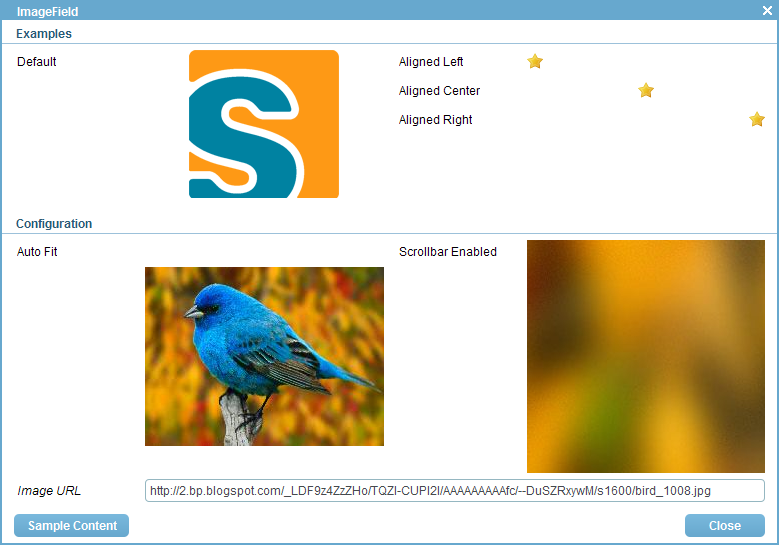
\includegraphics[width=14cm]{imagefield.png}
\caption{Image fields are used to display images and icons.
}
\figlabel{imagefield}
\end{figure}

\noindent Existing Documentation
\begin{itemize}
  \item forum: scrollbars \url{http://www.eclipse.org/forums/index.php/t/291205/}
\end{itemize}

% --------------------------------------------------------------------------- %
\section{SVG Field}
needs text

\begin{figure}
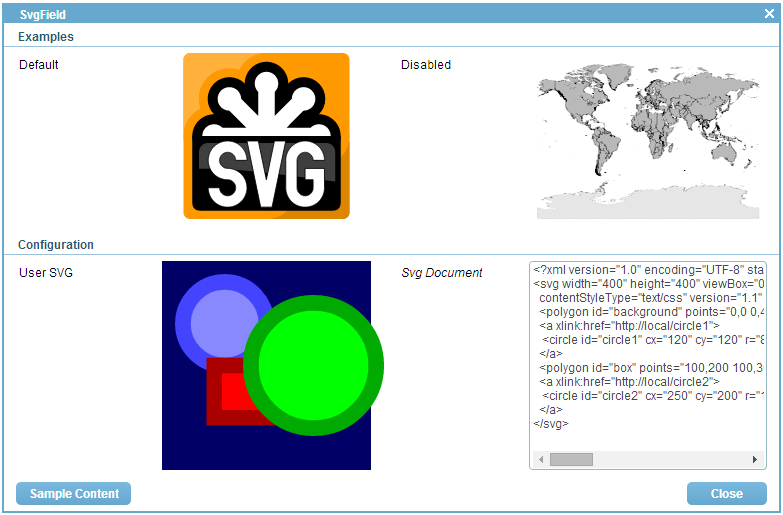
\includegraphics[width=15cm]{svgfield.png}
\caption{SVG fields and example use cases.
More text.}
\figlabel{svgfield}
\end{figure}

\noindent Existing Documentation
\begin{itemize}
  \item wiki tutorial \url{http://wiki.eclipse.org/Scout/Tutorial/3.8/SVG_Field}
\end{itemize}

% --------------------------------------------------------------------------- %
\section{HTML Field}
needs text

% --------------------------------------------------------------------------- %
\section{Browser Field}
needs text

\noindent Existing Documentation
\begin{itemize}
  \item forum: \url{http://www.eclipse.org/forums/index.php/t/414483/}, 
  \item forum: \url{http://www.eclipse.org/forums/index.php/t/369963/}, 
  \item forum: mozilla as default: \url{http://www.eclipse.org/forums/index.php/t/342433/}
\end{itemize}

% --------------------------------------------------------------------------- %
\section{Calendar Field}
needs text

\noindent Existing Documentation
\begin{itemize}
  \item forum: calendar field \url{http://www.eclipse.org/forums/index.php/t/370052/}
  \item forum: execloaditems \url{http://www.eclipse.org/forums/index.php/t/277447/}
  \item forum: filtering items \url{http://www.eclipse.org/forums/index.php/t/285644/}
  \item forum: usage example \url{http://www.eclipse.org/forums/index.php/t/265028/}
\end{itemize}

% =========================================================================== %
\chapter{Layout Widgets}
\chalabel{layoutwidgets}

% --------------------------------------------------------------------------- %
\section{Group Box}
needs text


\begin{figure}
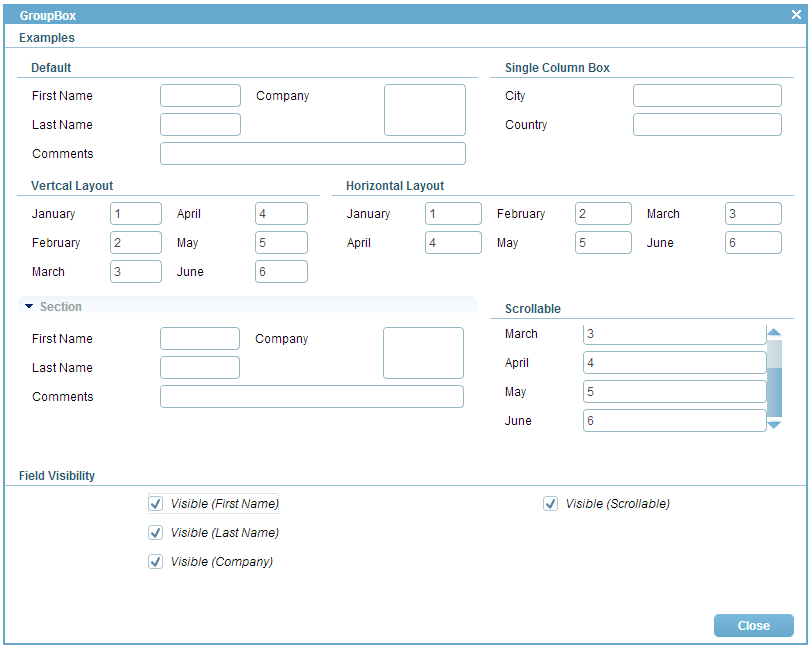
\includegraphics[width=15cm]{groupbox.png}
\caption{Group boxes and example use cases.
More text.}
\figlabel{groupbox}
\end{figure}

% --------------------------------------------------------------------------- %
\section{Tab Box}
needs text

\begin{figure}
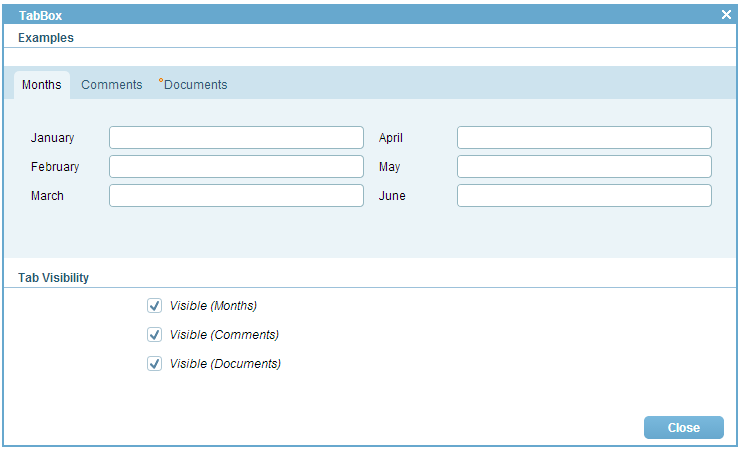
\includegraphics[width=15cm]{tabbox.png}
\caption{Tab boxes and example use cases.
More text.}
\figlabel{tabbox}
\end{figure}

% --------------------------------------------------------------------------- %
\section{Sequence Box}
needs text

\begin{figure}
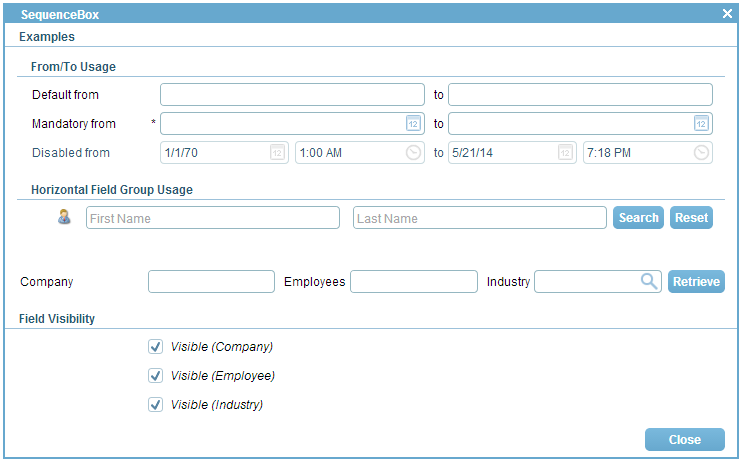
\includegraphics[width=15cm]{sequencebox.png}
\caption{Sequence boxes and example use cases.
More text.}
\figlabel{sequencebox}
\end{figure}

\noindent Existing Documentation
\begin{itemize}
  \item forum: \url{http://www.eclipse.org/forums/index.php/t/414629/}
\end{itemize}

* exec methods
* field validation

% --------------------------------------------------------------------------- %
\section{Split Box}
needs text

\begin{figure}
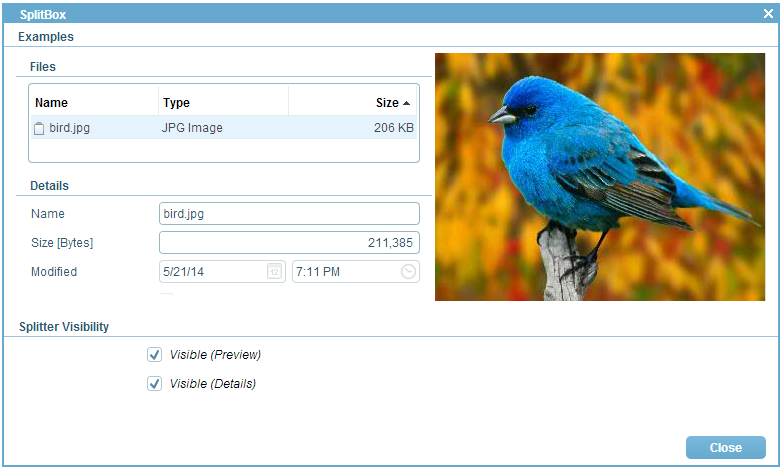
\includegraphics[width=15cm]{splitbox.png}
\caption{Split boxes and example use cases.
More text.}
\figlabel{splitbox}
\end{figure}


% --------------------------------------------------------------------------- %
\section{Page Field}
needs text

\noindent Existing Documentation
\begin{itemize}
  \item forum: \url{http://www.eclipse.org/forums/index.php/t/395360/}
\end{itemize}

% --------------------------------------------------------------------------- %
\section{File Chooser Field}
needs text

\noindent Existing Documentation
\begin{itemize}
  \item forum: file chooser field \url{http://www.eclipse.org/forums/index.php/t/377581/}
  \item forum: open with default file name: \url{http://www.eclipse.org/forums/index.php/t/351352/}
  \item how-to wiki: rap file chooser \url {http://wiki.eclipse.org/Scout/HowTo/3.8/Add_FileChooser_support_for_RAP_UI}
\end{itemize}

% --------------------------------------------------------------------------- %
\section{Master Slave Fields}
needs text

\noindent Existing Documentation
\begin{itemize}
  \item forum: \url{http://www.eclipse.org/forums/index.php/t/366931/}
\end{itemize}

% =========================================================================== %
\chapter{Custom Fields}
\chalabel{custom_fields}

As we have seen in the previous chapter, Scout already comes with a large amount of ready to use form fields. 
However, real life projects often need to meet special business requirements that can not be covered by the existing Scout form fields. 
For such situations the flexibility of the Scout framework allows the project to extend the exiting set of form fields with custom form fields. 

Custom form fields concists of a couple of components. Modeling and UI and registration and extension point?

\noindent Existing Documentation
\begin{itemize}
  \item how-to wiki: \url{http://wiki.eclipse.org/Scout/HowTo/3.8/Add_a_custom_GUI_component}
  \item forum: wrap existing javaview.de swing component \url{http://www.eclipse.org/forums/index.php/t/262755/}
\end{itemize}

  * concept
  * showcase: drawing application

% =========================================================================== %
\chapter{Template Fields}
needs text

\noindent Existing Documentation
\begin{itemize}
  \item concept wiki: \url{http://wiki.eclipse.org/Scout/Concepts/Template}
  \item forum: form data for template fields \url{http://www.eclipse.org/forums/index.php/t/261235/}
  \item forum: form ''modularisation'' \url{http://www.eclipse.org/forums/index.php/t/245857/}
\end{itemize}



% =========================================================================== %
\chapter{Layouting}
needs text

\noindent Existing Documentation
\begin{itemize}
  \item concept wiki \url{http://wiki.eclipse.org/Scout/Concepts/Client_Plug-In#Layouting}
\end{itemize}

% --------------------------------------------------------------------------- %
\section{The Desktop}
needs text

% --------------------------------------------------------------------------- %
\section{Form Layout}
needs text


% =========================================================================== %
\chapter{Bookmarks}
needs text

% =========================================================================== %
\chapter{Client Notification}
needs text

\noindent Existing Documentation
\begin{itemize}
  \item presentation: \url{http://wiki.eclipse.org/images/e/ea/20121022_BahBah_Slides.pdf}
  \item concept wiki: \url{http://wiki.eclipse.org/Scout/Concepts/Client_Notification}
  \item forum: \url{http://www.eclipse.org/forums/index.php/t/241053/}
\end{itemize}
      
% =========================================================================== %
\chapter{File Upload and Download}
needs text

\noindent Existing Documentation
\begin{itemize}
  \item how-to wiki: \url{http://wiki.eclipse.org/Scout/HowTo/3.8/Transfer_a_file_from_the_client_to_the_server}
  \item how-to wiki: \url{http://wiki.eclipse.org/Scout/HowTo/3.8/Use_RemoteFileService}
  \item forum with error message box exampl \url{http://www.eclipse.org/forums/index.php/t/441101/}
  \item forum: \url{http://www.eclipse.org/forums/index.php/t/368166/}
  \item forum: \url{http://www.eclipse.org/forums/index.php/t/366585/}
  \item forum: remotefileservice \url{http://www.eclipse.org/forums/index.php/t/266862/}
  \item forum: file download \url{http://www.eclipse.org/forums/index.php/t/263896/}
  \item forum: load \& display file \url{http://www.eclipse.org/forums/index.php/t/440934/}
\end{itemize}

% =========================================================================== %
\chapter{Application Branding}
needs text

\noindent Existing Documentation
\begin{itemize}
  \item forum: \url{http://www.eclipse.org/forums/index.php/t/373921/}
  \item forum: Splash \url{http://www.eclipse.org/forums/index.php/t/263003/}, 
  \item forum: Splash \url{http://www.eclipse.org/forums/index.php/t/164495/}
  \item forum: Login Box \url{http://www.eclipse.org/forums/index.php/t/417248/}
  \item forum: App Icon \url{http://www.eclipse.org/forums/index.php/t/263221/}
  \item forum: App Name \url{http://www.eclipse.org/forums/index.php/t/262121/}
  \item forum: Desktop \url{http://www.eclipse.org/forums/index.php/t/373921/}
  \item forum: Scout info form \url{http://www.eclipse.org/forums/index.php/t/236630/}
\end{itemize}

* Icons
* Fonts / Colors
* Look and Feel (Swing)

% --------------------------------------------------------------------------- %
\section{Rayo Look and Feel}
needs text

\noindent Existing Documentation
\begin{itemize}
  \item forum \url{http://www.eclipse.org/forums/index.php/t/369809/}
  \item wiki tutorial \url{http://wiki.eclipse.org/Scout/Tutorial/3.8/Rayo_Look_and_Feel}
\end{itemize}

% --------------------------------------------------------------------------- %
\section{Branding the Swing Client}
needs text

\noindent Existing Documentation
\begin{itemize}
  \item how-to wiki: for logo \url{http://wiki.eclipse.org/Scout/HowTo/3.8/Branding_the_Swing_Client}
  \item how-to wiki: app logo \url{http://wiki.eclipse.org/Scout/HowTo/3.8/Exchange_Default_Images}
\end{itemize}

% --------------------------------------------------------------------------- %
\section{Branding the SWT Client}
needs text

\noindent Existing Documentation
\begin{itemize}
  \item how-to wiki: for logo \url{http://wiki.eclipse.org/Scout/HowTo/3.8/Branding_the_Swing_Client}
  \item how-to wiki: app logo \url{http://wiki.eclipse.org/Scout/HowTo/3.8/Exchange_Default_Images}
\end{itemize}

% --------------------------------------------------------------------------- %
\section{Branding the Webclient}
needs text

\noindent Existing Documentation
\begin{itemize}
  \item forum \url{http://www.eclipse.org/forums/index.php/t/367983/}
\end{itemize}

% =========================================================================== %
\chapter{Advanced Topics}
needs text  

% --------------------------------------------------------------------------- %
\section{Modifying the UI at Runtime}
needs text

\noindent Existing Documentation
\begin{itemize}
  \item forum: inject fields in form \url{http://www.eclipse.org/forums/index.php/t/367124/}
\end{itemize}

% --------------------------------------------------------------------------- %
\section{Focus Handling}
needs text

\noindent Existing Documentation
\begin{itemize}
  \item forum: \url{http://www.eclipse.org/forums/index.php/t/369585/}
\end{itemize}

% --------------------------------------------------------------------------- %
\section{Keyboard Control}
needs text

\noindent Existing Documentation
\begin{itemize}
  \item forum: \url{http://www.eclipse.org/forums/index.php/t/351417/}
\end{itemize}

% --------------------------------------------------------------------------- %
\section{Master Detail Pages}
needs text

\noindent Existing Documentation
\begin{itemize}
  \item \url{http://www.eclipse.org/forums/index.php/t/405999/}
\end{itemize}

% --------------------------------------------------------------------------- %
\section{Client Only Applications}
needs text

\noindent Existing Documentation
\begin{itemize}
  \item how-to wiki: \url{http://wiki.eclipse.org/Scout/HowTo/3.8/Create_a_Standalone_Client_with_DB_Access}
  \item forum: client only \url{http://www.eclipse.org/forums/index.php/t/210183/}
  \item forum: offline capable client \url{http://www.eclipse.org/forums/index.php/t/210183/}
\end{itemize}


% --------------------------------------------------------------------------- %
\section{Headless Client}
needs text

\noindent Existing Documentation
\begin{itemize}
  \item headless client forum \url{http://www.eclipse.org/forums/index.php/t/262563/}
\end{itemize}

% --------------------------------------------------------------------------- %
\section{Client Startup}
needs text

\noindent Existing Documentation
\begin{itemize}
  \item reading command line parameters forum \url{http://www.eclipse.org/forums/index.php/t/281816/}
  \item do something right after login forum \url{http://www.eclipse.org/forums/index.php/t/261999/}
\end{itemize}

\subsection{Config.ini File}
needs text

\noindent Existing Documentation
\begin{itemize}
  \item config ini file forum \url{http://www.eclipse.org/forums/index.php/t/365140/}
  \item os independent *product/confg.ini forum \url{http://www.eclipse.org/forums/index.php/t/261674/}
\end{itemize}

% --------------------------------------------------------------------------- %
\section{Client Shutdown}
needs text

% --------------------------------------------------------------------------- %
\section{Threading and Jobs}
needs text

\noindent Existing Documentation
\begin{itemize}
  \item threading and jobs concept wiki \url{http://wiki.eclipse.org/Scout/Concepts/Client_Plug-In#Threading_and_Jobs}
\end{itemize}


% --------------------------------------------------------------------------- %
\section{Caching}
needs text

% --------------------------------------------------------------------------- %

\ifx\wholebook\relax\else
   \begin{thebibliography}{99}
  \addcontentsline{toc}{chapter}{Bibliography}
  
  % add/insert books in alphabetical order of 1st author
  
  \bibitem{batessierra05}
    \textit{Bert Bates, Kathy Sierra},
	\textbf{Head First Java} 2nd edition, 
	O'Reilly Media, 2005.

  \bibitem{bloch08} 
    \textit{Joshua Bloch},
    \textbf{Effective Java} 2nd edition, 
	Addison-Wesley, 2008.
	
  \bibitem{eckel06}
    \textit{Bruce Eckel},
	\textbf{Thinking in Java} 4th edition, 
	Prentice Hall International, 2006.

\end{thebibliography}

   \end{document}
\fi

% =========================================================================== %
